\documentclass{article}
\usepackage{graphicx} % Required for inserting images
\usepackage{float}

\title{Kuwahara filter with GPU}
\author{Hai Nguyen Ngoc}
\date{November 2024}

\begin{document}

\maketitle

\section{Introduction}
This project apply Kuwahara for images to compare the performance of CPU, GPU with and without shared memory.
\section{Implementation}
\subsection{CPU}
First, program need to loads an image from a specified path and converts it into a format that the program can work with. The image is then transformed from RGB (red, green, blue) color space to HSV (hue, saturation, value) color space. The Kuwahara filter is applied to the HSV image. Then program chooses the section with the least variation in color, which helps to reduce noise and create a smoother appearance. Finally, the processed image is converted back to RGB format, displayed, and the time taken to complete the filtering process is printed. The result is a visually appealing image that retains important features while reducing unwanted noise.
\subsection{GPU without shared memory}
Do the same mission with the CPU program, but need to run by cuda. The data in the process of this program is loaded directly from memory of the GPU, without shared memory. The GPU can handle thousands of threads simultaneously, allowing for much faster processing of each pixel in the image. This parallelism greatly reduces the time required for both the color conversion and the filtering operations.  \\
In the no shared memory version, data in the kernel is read from data in the data in each thread without shared memory.
\subsection{GPU with shared memory}
Do the same mission with 2 above program, but using shared memory for the data of the program. It means that the data in the shared memory is accessed several times. Theoretically, this process will help program reduce execution time by reducing reading data from memory many times. \\
Shared memory is declared and used for several time, instead of reading from tidx and tidy.
\section{Result}
\subsection{The result of Kuwahara filter}
\begin{figure} [H]
    \centering
    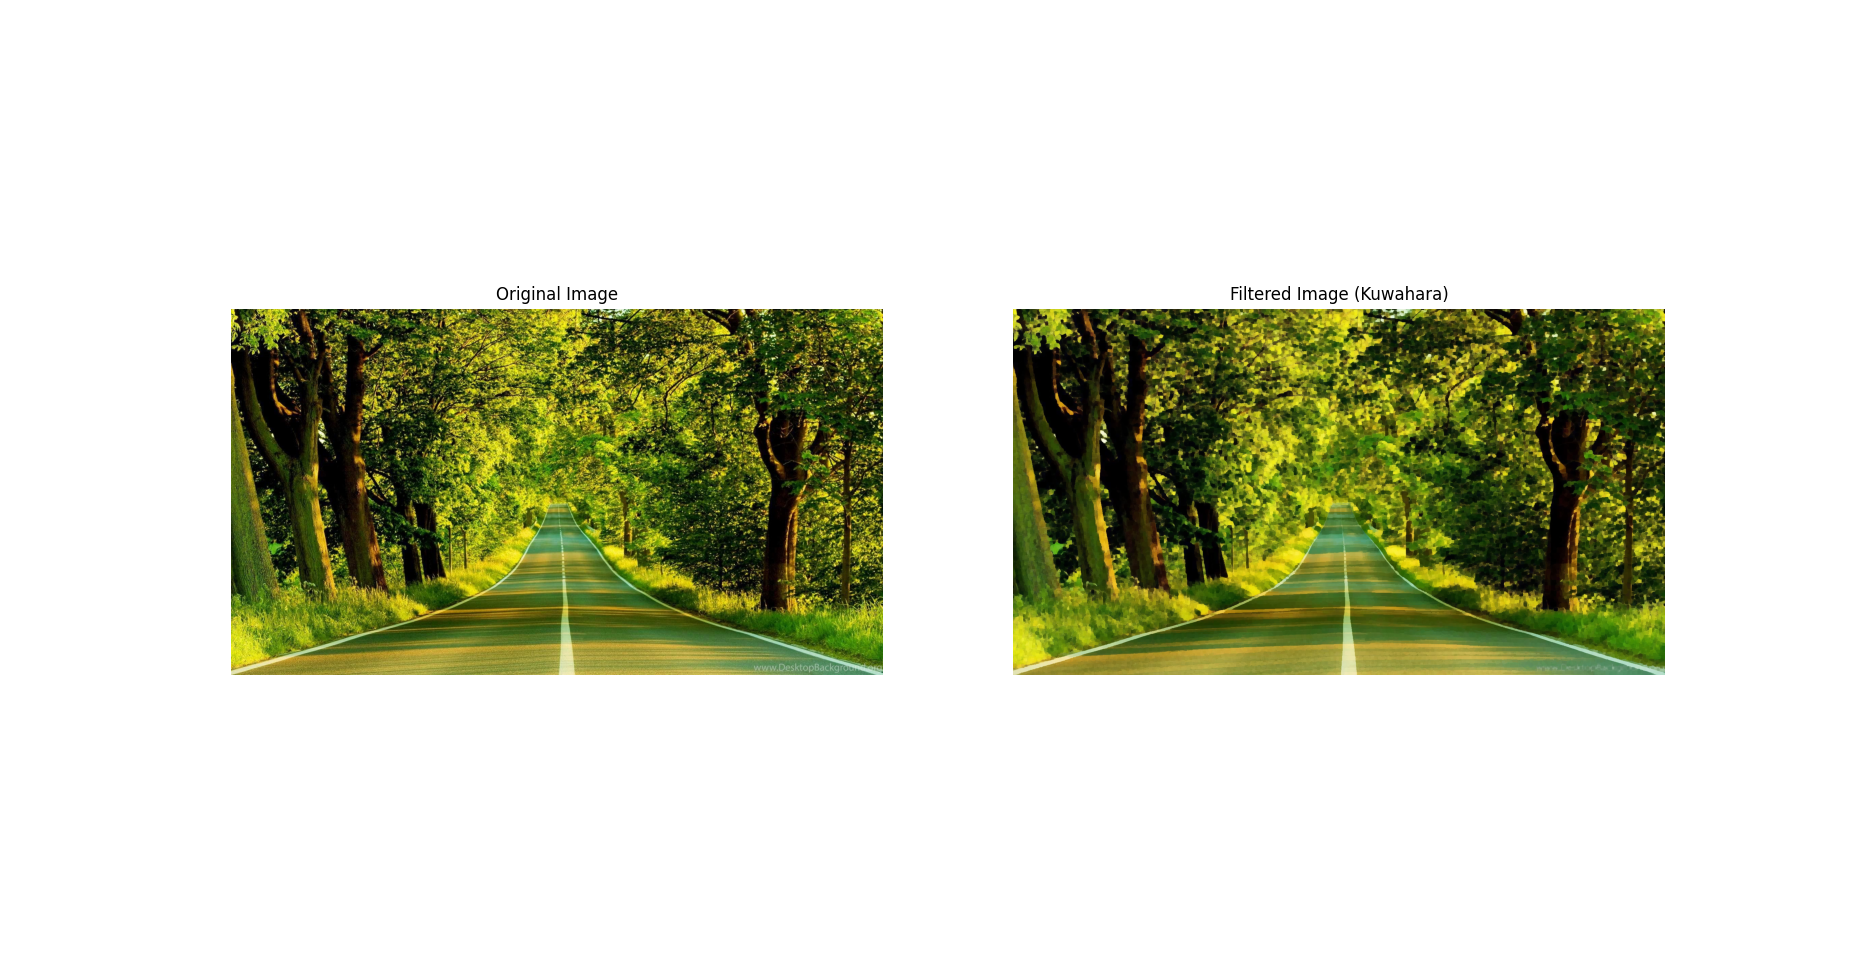
\includegraphics[width=1\linewidth]{input_output.png}
    \caption{Input of programs}
    \label{fig:enter-label}
\end{figure}
The output is respected to the algorithms of Kuwahara filter (edge preservation, noise reduction, adaptive smoothing)
\subsection{The comparison of performance}
The execution time of CPU is too large (more than 1 minute), so I did not add to the graph to make comparison for better visualization.
\begin{figure} [H]
    \centering
    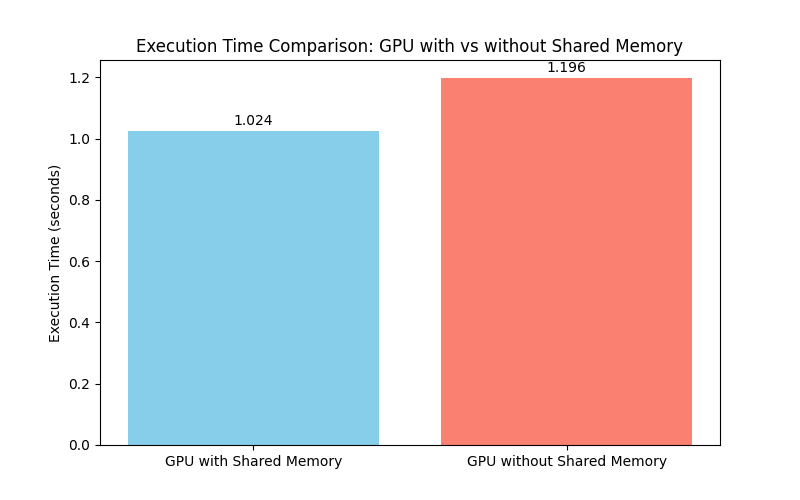
\includegraphics[width=1\linewidth]{comparison.png}
    \caption{Comparison of shared memory versus no shared memory in execution time}
    \label{fig:enter-label}
\end{figure}
The execution time of Shared memory is faster than no shared memory. It proved the efficiency of shared memory in the performance of program. Shared memory help to reduce latency of reading data in GPU - which make GPU run lower.
\subsection{Conclusion}
In this project of the Kuwahara filter, It is easy to observe that using the GPU instead of the CPU makes a big difference in processing speed. The CPU version took the longest time to run, showing it’s not the best choice for this type of task. Switching to the GPU provided a large speedup, and using shared memory on the GPU made it even faster by improving how data is accessed. This shows that shared memory can be very useful for making GPU processing more efficient. Overall,to get the best performance in image processing tasks, shared memory in GPU implementations should be used.
\end{document}
